% Digital Logic Report Template
% Created: 2020-01-10, John Miller

%==========================================================
%=========== Document Setup  ==============================

% Formatting defined by class file
\documentclass[11pt]{article}

% ---- Document formatting ----
\usepackage[margin=1in]{geometry}	% Narrower margins
\usepackage{booktabs}				% Nice formatting of tables
\usepackage{graphicx}				% Ability to include graphics

%\setlength\parindent{0pt}	% Do not indent first line of paragraphs 
\usepackage[parfill]{parskip}		% Line space b/w paragraphs
%	parfill option prevents last line of pgrph from being fully justified

% Parskip package adds too much space around titles, fix with this
\RequirePackage{titlesec}
\titlespacing\section{0pt}{8pt plus 4pt minus 2pt}{3pt plus 2pt minus 2pt}
\titlespacing\subsection{0pt}{4pt plus 4pt minus 2pt}{-2pt plus 2pt minus 2pt}
\titlespacing\subsubsection{0pt}{2pt plus 4pt minus 2pt}{-6pt plus 2pt minus 2pt}

% ---- Hyperlinks ----
\usepackage[colorlinks=true,urlcolor=blue]{hyperref}	% For URL's. Automatically links internal references.

% ---- Code listings ----
\usepackage{listings} 					% Nice code layout and inclusion
\usepackage[usenames,dvipsnames]{xcolor}	% Colors (needs to be defined before using colors)

% Define custom colors for listings
\definecolor{listinggray}{gray}{0.98}		% Listings background color
\definecolor{rulegray}{gray}{0.7}			% Listings rule/frame color

% Style for Verilog
\lstdefinestyle{Verilog}{
	language=Verilog,					% Verilog
	backgroundcolor=\color{listinggray},	% light gray background
	rulecolor=\color{blue}, 			% blue frame lines
	frame=tb,							% lines above & below
	linewidth=\columnwidth, 			% set line width
	basicstyle=\small\ttfamily,	% basic font style that is used for the code	
	breaklines=true, 					% allow breaking across columns/pages
	tabsize=3,							% set tab size
	commentstyle=\color{gray},	% comments in italic 
	stringstyle=\upshape,				% strings are printed in normal font
	showspaces=false,					% don't underscore spaces
}

% How to use: \Verilog[listing_options]{file}
\newcommand{\Verilog}[2][]{%
	\lstinputlisting[style=Verilog,#1]{#2}
}


\usepackage[section]{placeins}

%======================================================
%=========== Body  ====================================
\begin{document}

\title{ELC 2137 Lab 9: ALU with Input Register}
\author{Aaron Mendoza}

\maketitle


\section*{Summary}

Type the summary of your experiment and results here.  





\section*{Results}

\subsection*{Expected Results Tables}

\begin{table*}[ht]\centering
	\caption{\textit{register} expected results table}
	\label{ALU:tbl:register_ERT}\medskip
	\begin{tabular}{l|rrrrrrrrrrr}
		Time (ns): & 0-5 & 5-10 & 10-15 & 15-20 & 20-25 & 25-30 & 30-35 & 35-40 & 40-45 & 45-50 & 50-55 \\
		\midrule
		D (hex) & 0 & 0 	  & A & A & 3 	    & 3 	  & 0 	    & 0 & 0$\to$6 & 6 & 6 \\
		clk     & 0 & 1 	  & 0 & 1 & 0 	    & 1 	  & 0 	    & 1 & 0 	  & 1 & 0 \\
		en  	& 0 & 0 	  & 1 & 1 & 1$\to$0 & 0$\to$1 & 1$\to$0 & 0 & 0$\to$1 & 1 & 1 \\
		rst 	& 0 & 0$\to$1 & 0 & 0 & 0 		& 0 	  & 0		& 0 & 0		  & 0 & 0 \\
		\midrule
		Q (hex) & X & X$\to$0 & 0 & 0$\to$A & A & A & A & A & A & A$\to$6 & 6\\
		\bottomrule
	\end{tabular}
\end{table*}
\FloatBarrier

\begin{table*}[ht]\centering
	\caption{\textit{alu} expected results table skeleton}
	\label{ALU:tbl:alu_ERT}\medskip
	\begin{tabular}{l|rrrrrr}
		Time (ns): & 0-10 & 10-20 & 20-30 & 30-40 & 40-50 & 50-60 \\
		\midrule
		in0 & A & A & A & A & A & A \\
		in1 & 7 & 7 & 7 & 7 & 7 & 7 \\
		op	& 0 & 1 & 2 & 3 & 4 & default \\
		\midrule
		out & 17 & 3 & 2 & 15 & 13 & 10 \\
		\bottomrule
	\end{tabular}
\end{table*}

\subsection*{Simulation Waveforms}
\begin{figure}[ht]\centering
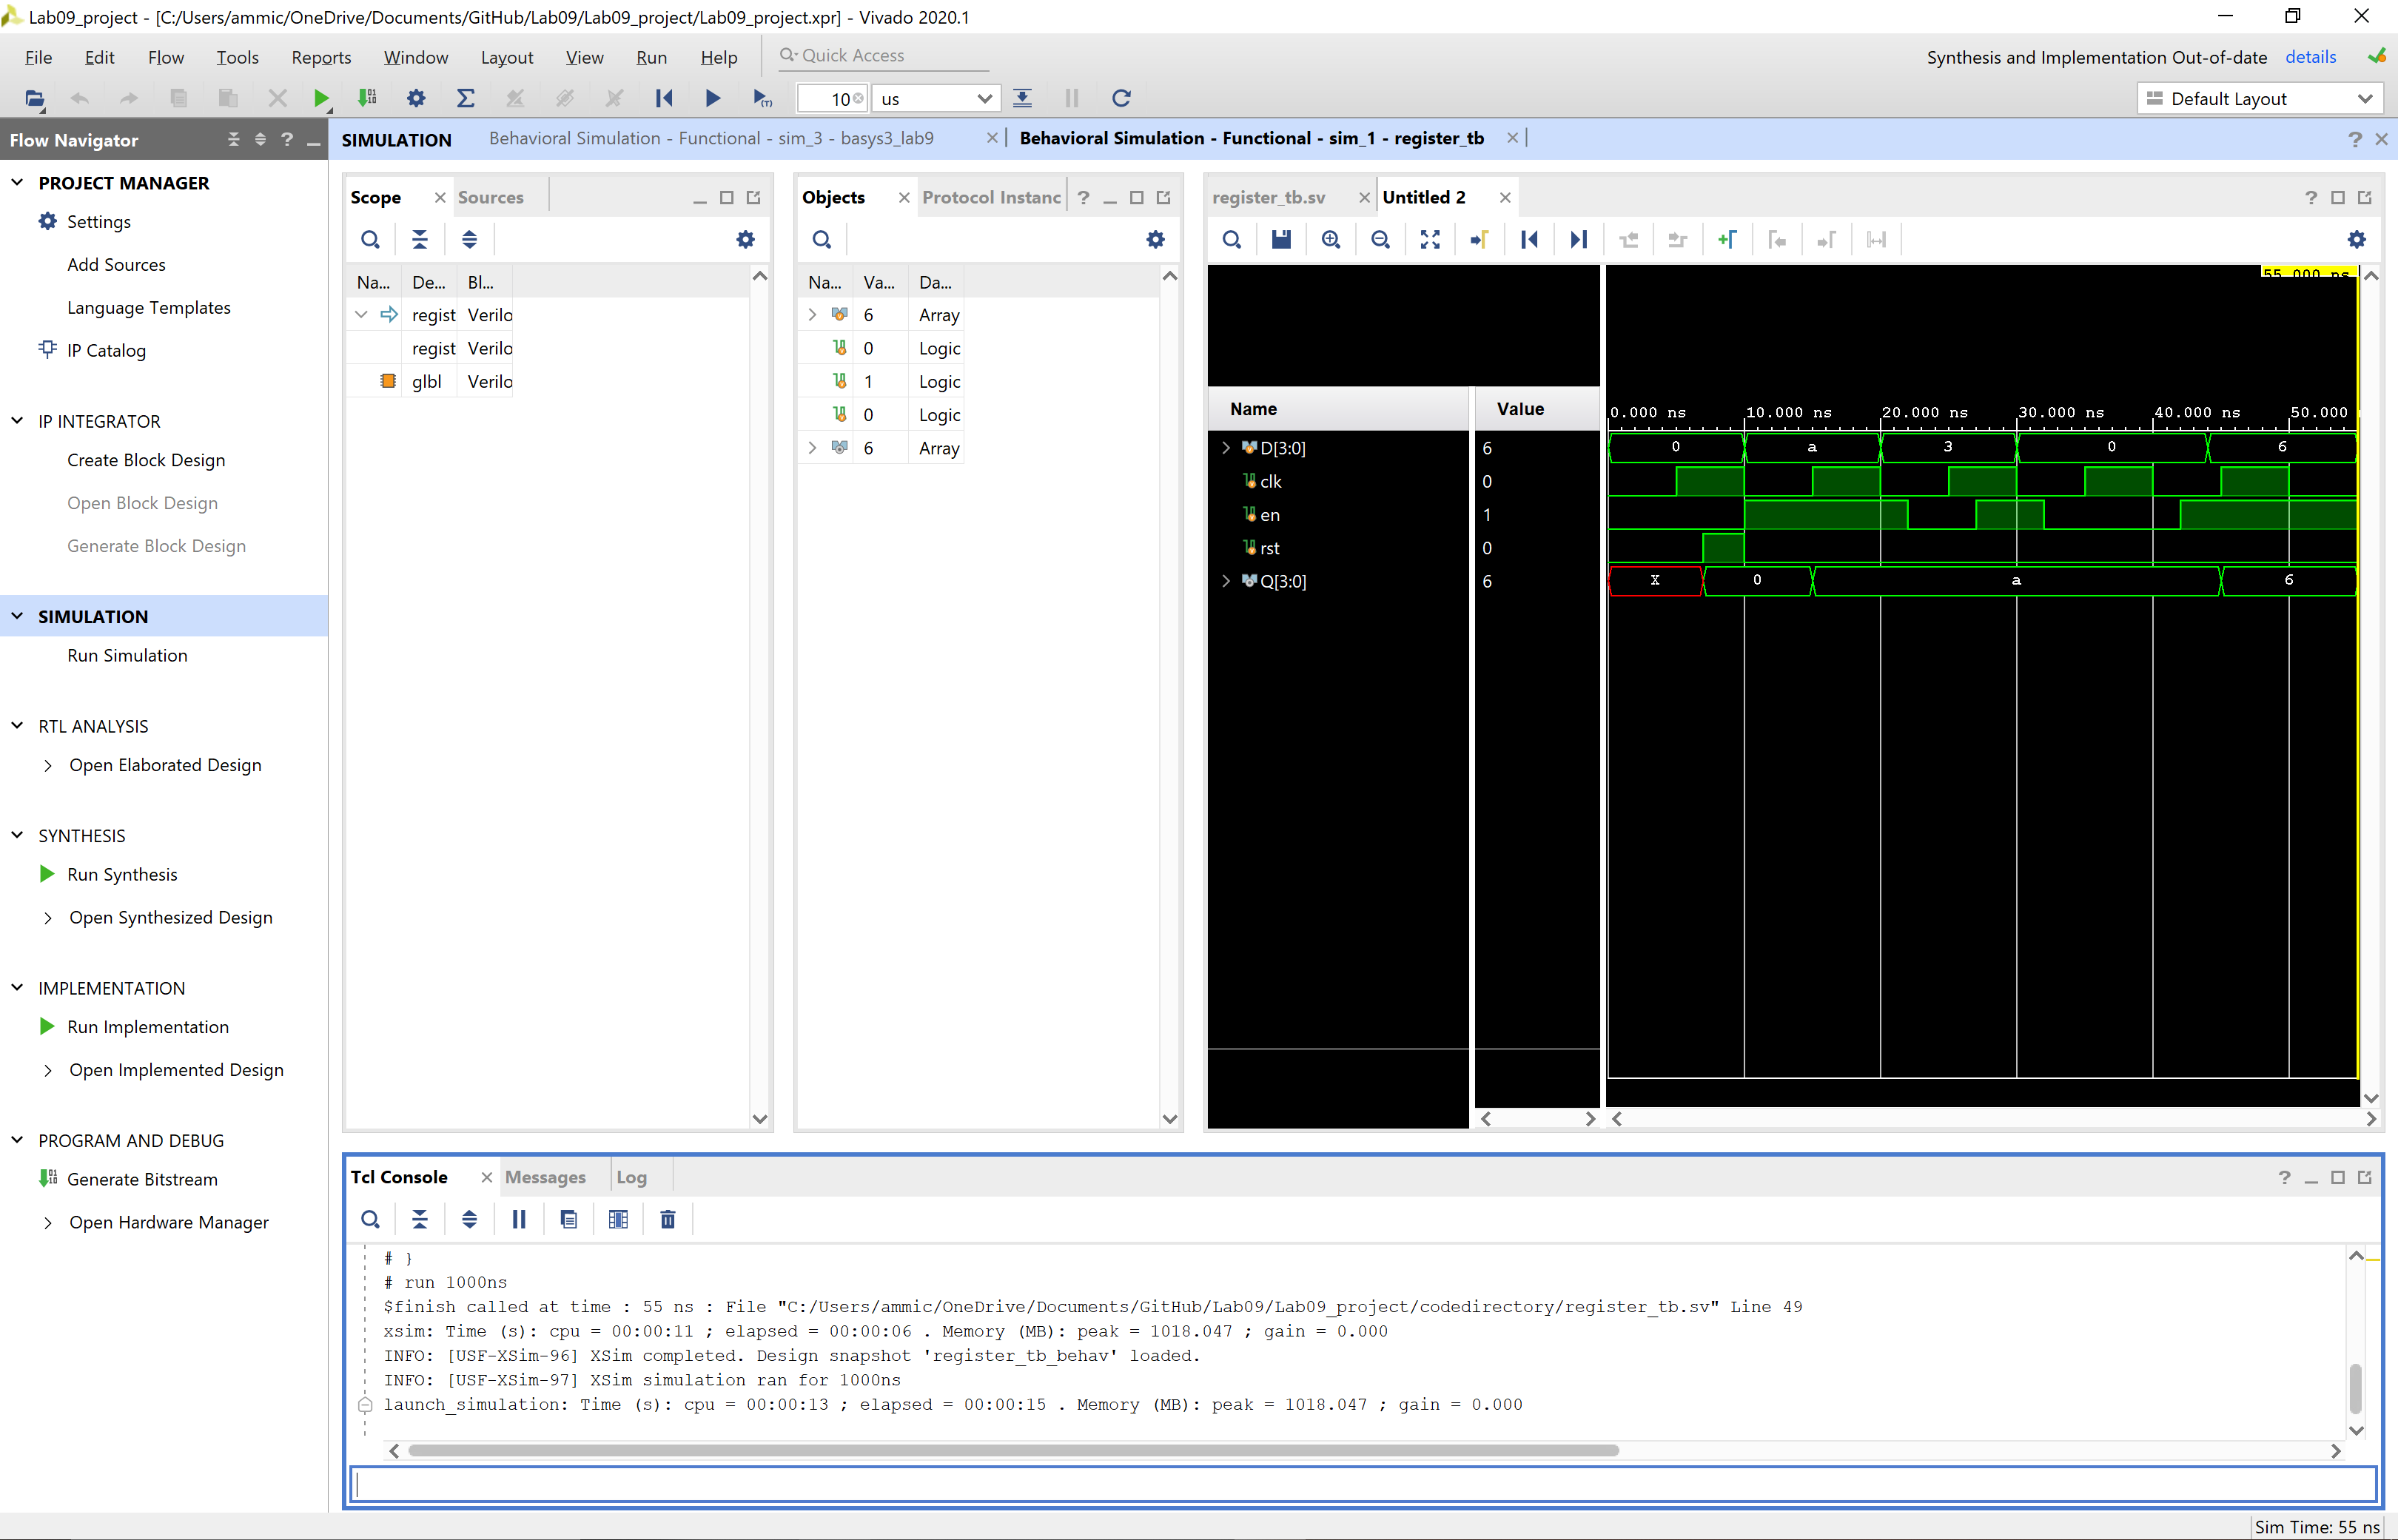
\includegraphics[width=1\textwidth,trim=19cm 15cm 0.5cm 4.5cm,clip]{register_tb_screenshot}
	\caption{Register Testbench Simulation}
	\label{fig:sim_with_table}
\end{figure}

\begin{figure}[ht]\centering
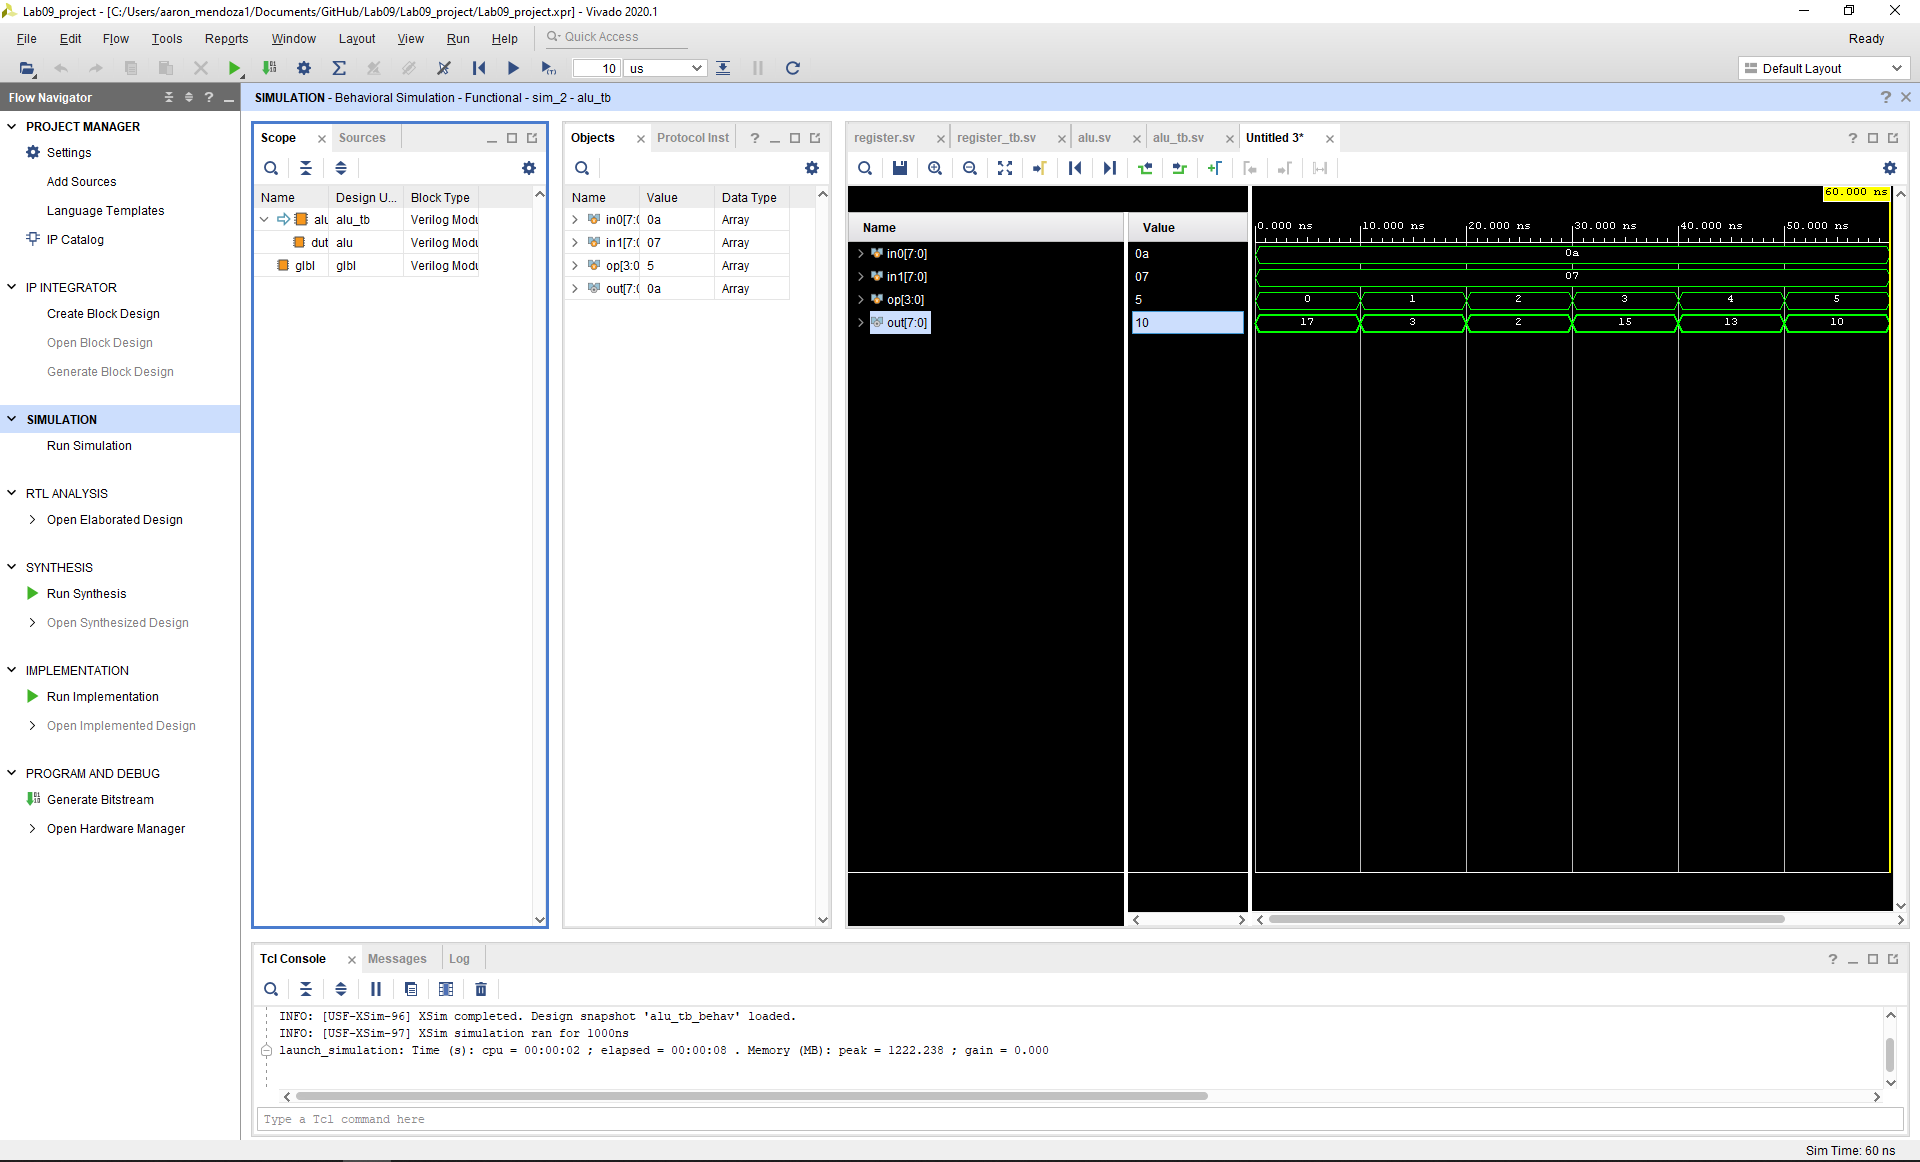
\includegraphics[width=1\textwidth,trim=19cm 15cm 0.5cm 4.5cm,clip]{alu_tb_screenshot}
	\caption{ALU Testbench Simulation}
	\label{fig:sim_with_table}
\end{figure}


\begin{figure}[ht]\centering
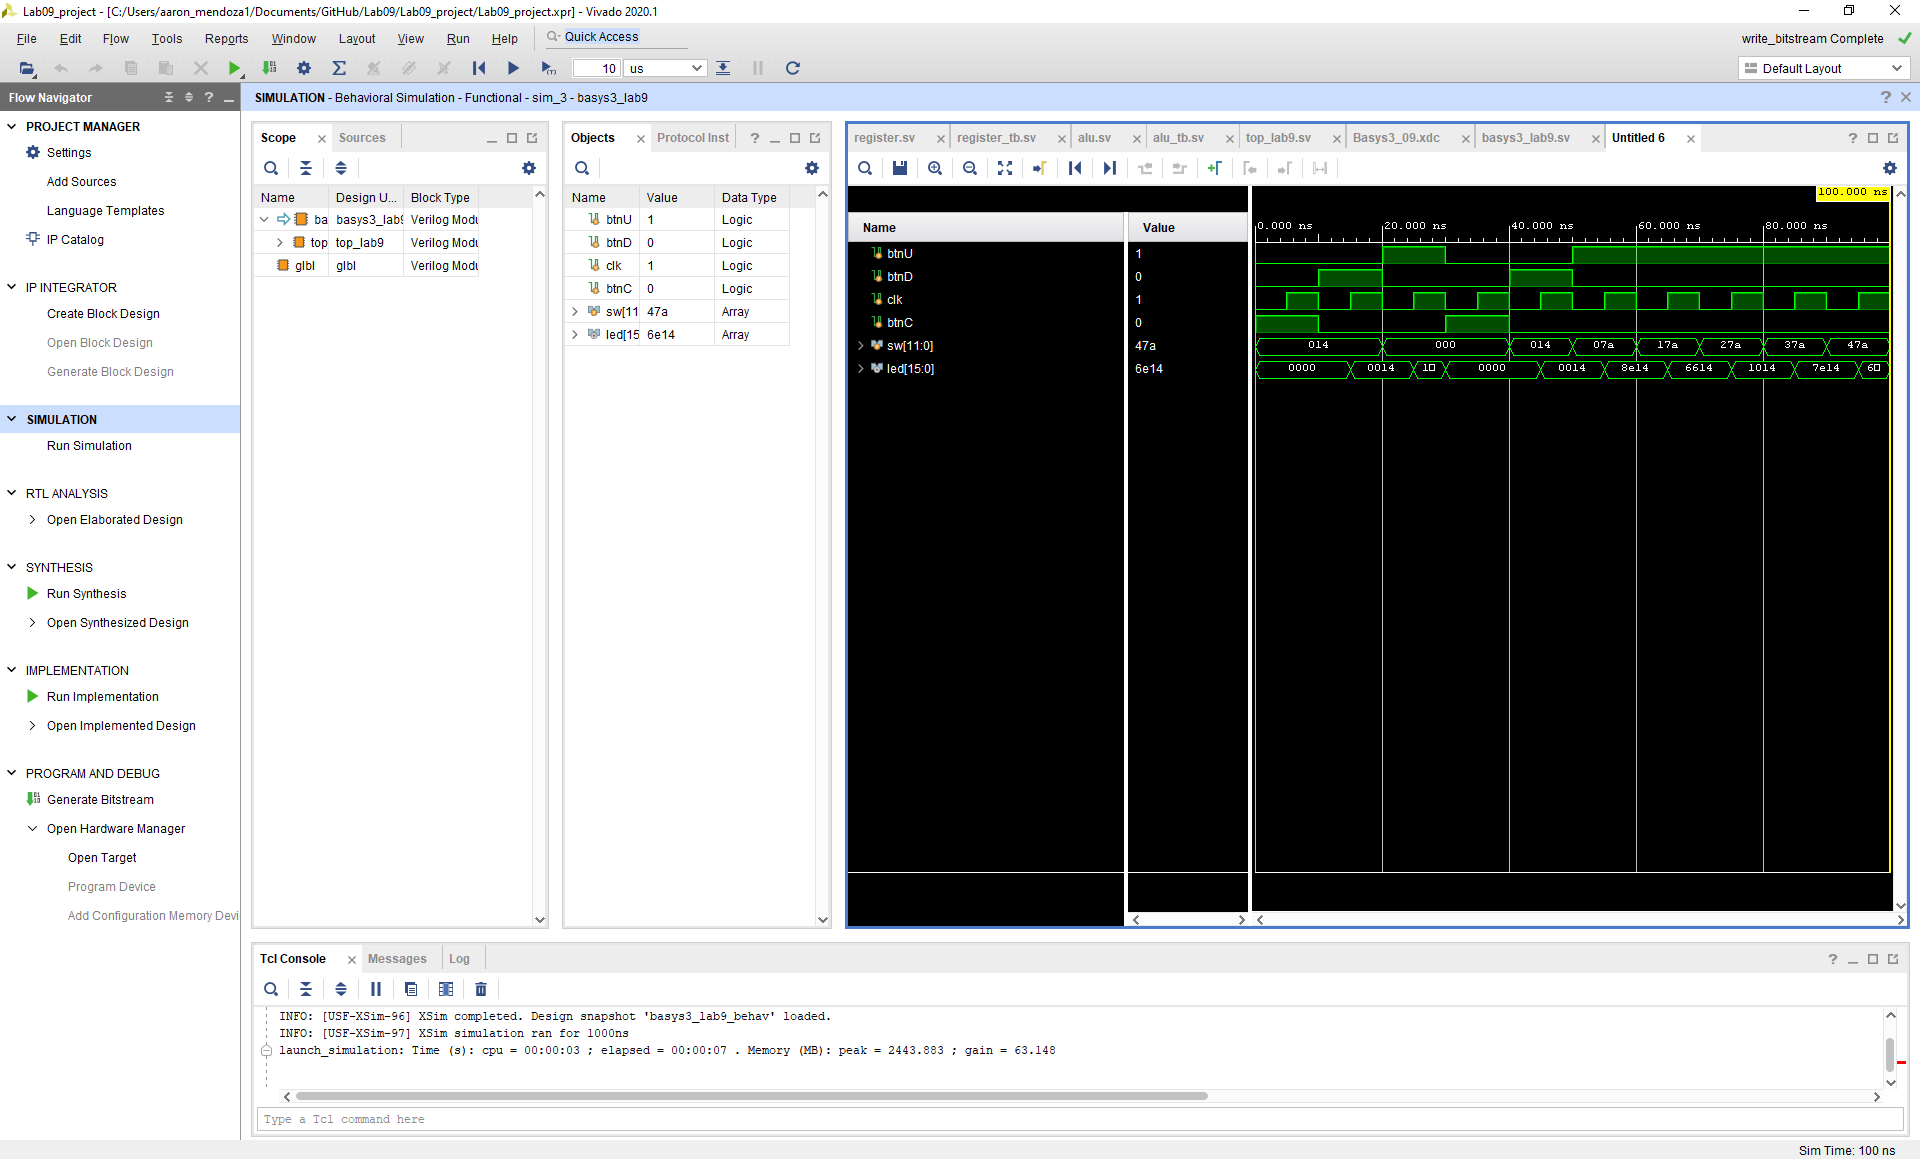
\includegraphics[width=1\textwidth,trim=19cm 15cm 0.5cm 4.5cm,clip]{top_level_sim}
	\caption{Top-Level Simulation}
	\label{fig:sim_with_table}
\end{figure}

\subsection*{Basys3 Board Pictures}

\begin{figure}[ht]\centering
\includegraphics[width=1\textwidth,trim=15cm 15cm 0.5cm 4.5cm,clip]{add}
	\caption{LEDs after Adding 8-bit hexadecimal 14 and 7A}
	\label{fig:sim_with_table}
\end{figure}

\begin{figure}[ht]\centering
\includegraphics[width=1\textwidth,trim=15cm 15cm 0.5cm 4.5cm,clip]{subtract}
	\caption{LEDs after Subtracting 8-bit hexadecimal 14 and 7A}
	\label{fig:sim_with_table}
\end{figure}

\begin{figure}[ht]\centering
\includegraphics[width=1\textwidth,trim=15cm 15cm 0.5cm 4.5cm,clip]{and}
	\caption{LEDs after "AND"ing 8-bit hexadecimal 14 and 7A}
	\label{fig:sim_with_table}
\end{figure}

\begin{figure}[ht]\centering
\includegraphics[width=1\textwidth,trim=15cm 15cm 0.5cm 4.5cm,clip]{or}
	\caption{LEDs after "OR"ing  8-bit hexadecimal 14 and 7A}
	\label{fig:sim_with_table}
\end{figure}

\begin{figure}[ht]\centering
\includegraphics[width=1\textwidth,trim=15cm 15cm 0.5cm 4.5cm,clip]{xor}
	\caption{LEDs after "XOR"ing 8-bit hexadecimal 14 and 7A}
	\label{fig:sim_with_table}
\end{figure}

\begin{figure}[ht]\centering
\includegraphics[width=1\textwidth,trim=15cm 15cm 0.5cm 4.5cm,clip]{default}
	\caption{LEDs after putting default operation of 8-bit hexadecimal 14 and 7A}
	\label{fig:sim_with_table}
\end{figure}

\section*{Code}

\Verilog[firstline=22, lastline=37, caption=Register Module Code]{Lab09_project/codedirectory/register.sv}|

\Verilog[firstline=22, lastline=53, caption=Register Testbench Code]{Lab09_project/codedirectory/register_tb.sv}|

\Verilog[firstline=22, lastline=49, caption=ALU Module Code]{Lab09_project/codedirectory/alu.sv}|

\Verilog[firstline=22, lastline=47, caption=ALU Testbench Code]{Lab09_project/codedirectory/alu_tb.sv}|

\Verilog[firstline=22, lastline=58, caption=Top Level Module Code]{Lab09_project/codedirectory/top_lab9.sv}|


\end{document}
